\documentclass{article}
\usepackage{graphicx}
\graphicspath{ {images/} }

% Math-mode symbol & verbatim
\def\W#1#2{$#1{#2}$ &\tt\string#1\string{#2\string}}
\def\X#1{$#1$ &\tt\string#1}
\def\Y#1{$\big#1$ &\tt\string#1}
\def\Z#1{\tt\string#1}
 
\newcommand\tab[1][1cm]{\hspace*{#1}}

\begin{document}

\title{%
  Nature Inspired Search and Optimisation  \\
  \large Exercise 2 \\
    }

\author{1429527}

\maketitle

\section{For a multi-objective optimisation problem, what is the difference between Pareto-optimal solutions and Pareto-optimal front?}

Pareto-optimal front is a curve of non-dominated points, with respect to the objectives, on the boundary of the feasible region. There are infinite points on this front of optimal solutions and so infinite solutions. 

Pareto-optimal solutions are specified points on the Pareto-optimal front. These solutions maximise the objectives.

\section{}

\begin{center}
\begin{tabular}{ |c|c|c|c|c|c|c|c|c|c| } 
 \hline
 $x_1$ & $x_2$ & $x_3$ & $x_4$ & $x_5$ & $y_1$ & $y_2$ & $y_3$ & $y_4$ & $y_5$ \\ 
 (11,7) & (8,5) & (13,15) & (10,17) & (9,9) & (6,7) & (14,6) & (15,12) & (12,13) & (16,9) \\
 \hline
\end{tabular}
\end{center}

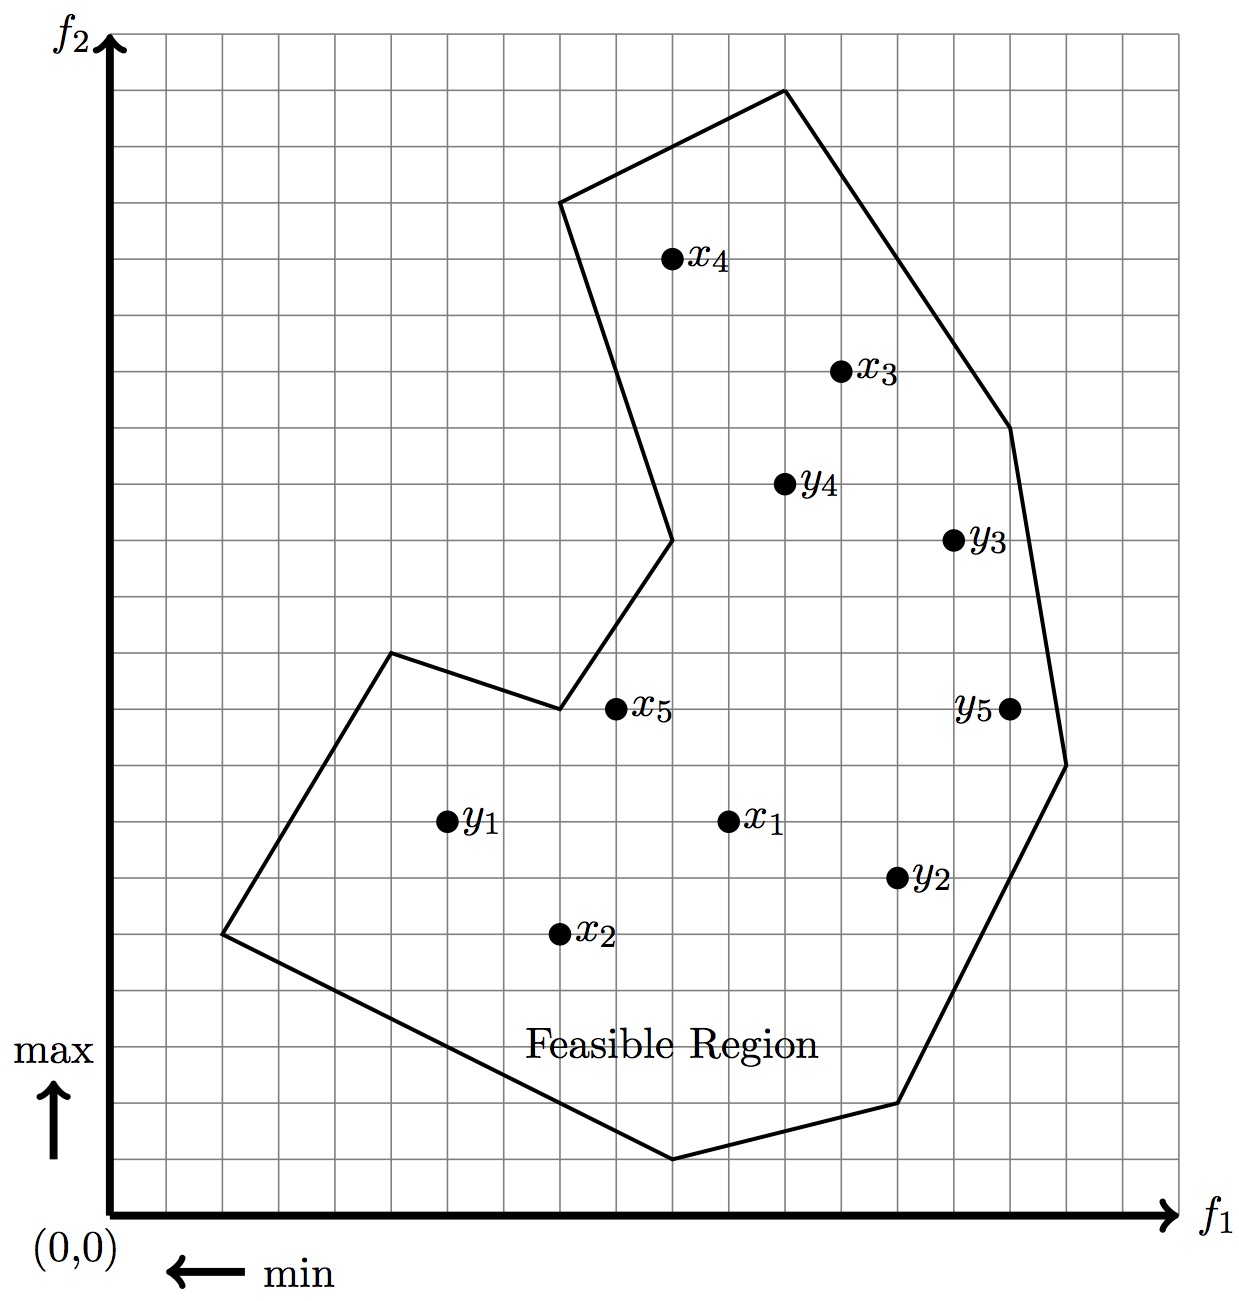
\includegraphics[width=10cm,height=10cm,keepaspectratio]{fig1.jpg}

\subsection{Identify the Pareto-optimal front of the above bi-objective problem by drawing it on the figure}

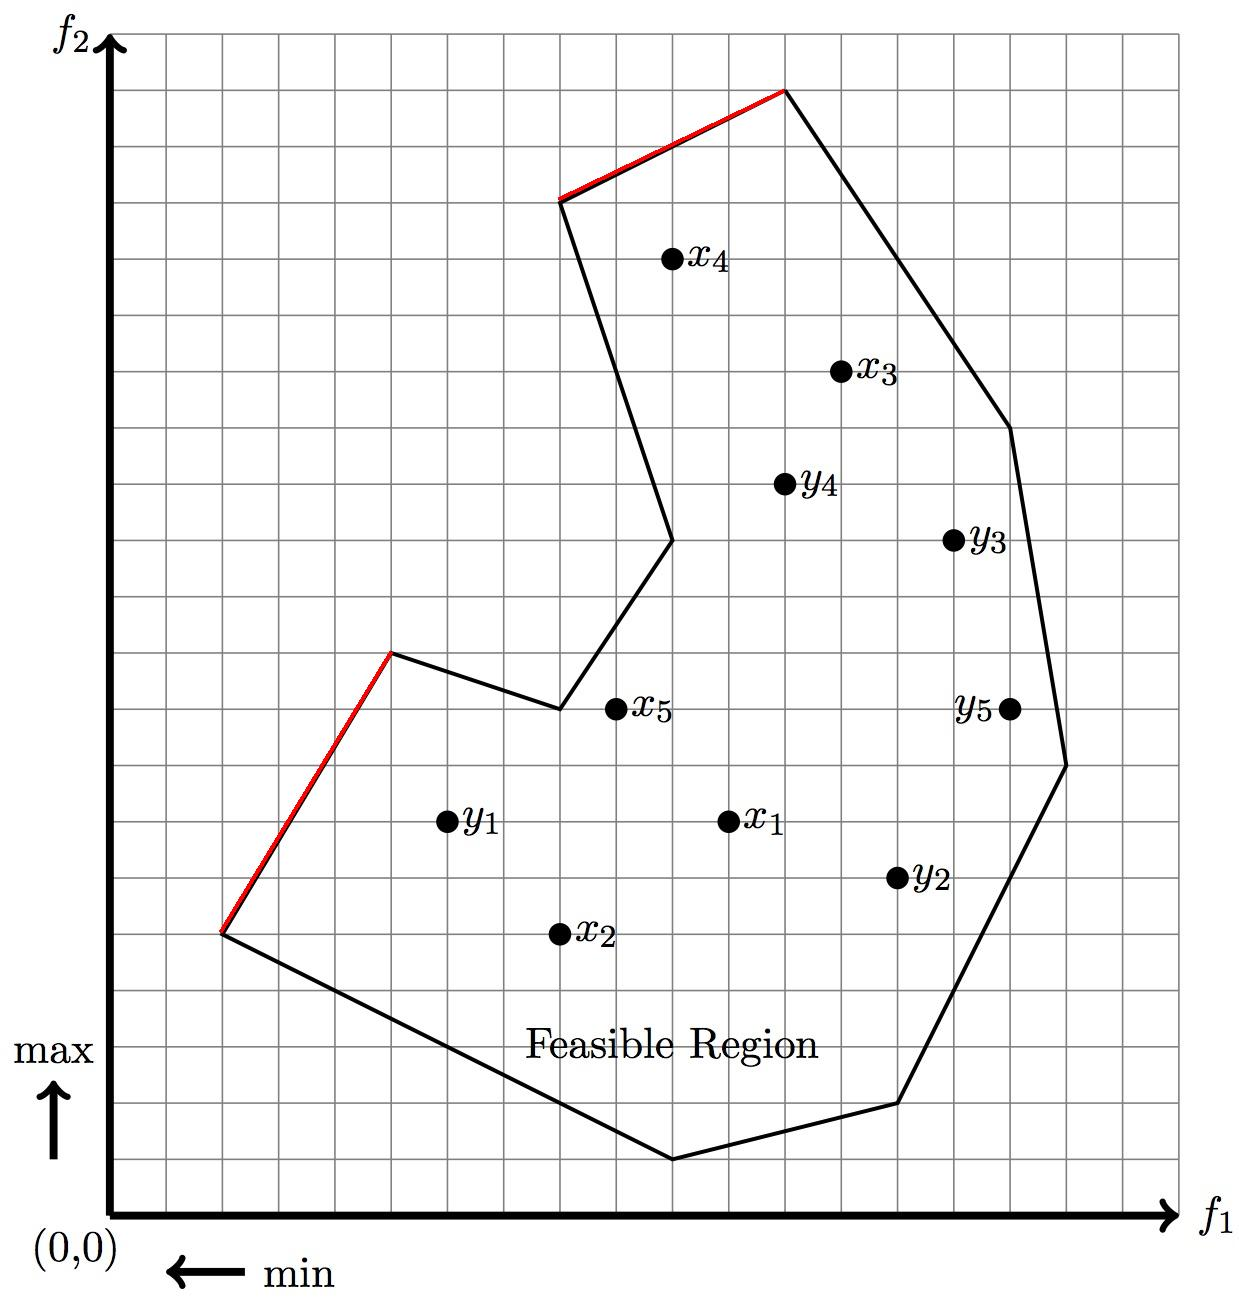
\includegraphics[width=10cm,height=10cm,keepaspectratio]{optFront}

\subsection{Consider search point $y_4$. For each of the other search points, state if $y_4$ dominates the point, is
dominated by the point or is incomparable to the point}

\begin{center}
\begin{tabular}{ |c|c| } 
 \hline
 $x_1$ & Incomparable \\ 
 \hline
 $x_2$ & Incomparable\\ 
 \hline
 $x_3$ & Incomparable \\ 
 \hline
 $x_4$ & Dominates $y_4$ \\ 
 \hline
 $x_5$ & Incomparable \\ 
 \hline
 $y_1$ & Incomparable \\ 
 \hline
 $y_2$ & Dominated by $y_4$ \\ 
 \hline
 $y_3$ & Dominated by $y_4$ \\  
 \hline
 $y_5$ & Dominated by $y_4$ \\ 
 \hline
\end{tabular}
\end{center}

\subsection{NSGA-II [1] uses non-dominated sorting to divide the population into different non-dominated
classes of solutions. Perform this step of NSGA-II for the given individuals. For each of the individuals
indicate its class number, where the best class has number 0}

Implementing the fast-non-dominated-sort algorithm on page 184 of [1].
\smallbreak
For each individual, find the items that it dominates and is dominated by.
\bigbreak
$\mathcal{F}_1$ = $\O$
\bigbreak

For $x_1$
\smallbreak
 $S_{x_1}$ = \{$y_2$\}\tab Set dominated by $x_1$.
\smallbreak
 $n_{x_1}$ =  3\tab \tab Domination Counter - number of solutions $x_1$ is dominated by.

\bigbreak

 $S_{x_2}$ = \{\} 	
\smallbreak
 $n_{x_2}$ = 1	
\bigbreak
 $S_{x_3}$ = \{$y_2$, $y_3$, $y_5$\} 	
\smallbreak
 $n_{x_3}$ = 1	
\bigbreak
 $S_{x_4}$ = \{$x_1$, $x_3$, $y_2$, $y_3$, $y_4$, $y_5$\} 	
\smallbreak
 $n_{x_4}$ = 0	
\bigbreak
 $x_{4_{rank}}$ = 1
\smallbreak
 $\mathcal{F}_1$ = \{$x_4$\}
\bigbreak
 $S_{x_5}$ = \{$x_1$, $y_2$, $y_5$\} 	
\smallbreak
 $n_{x_5}$ = 0
\bigbreak
 $x_{5_{rank}}$ = 1
\smallbreak
 $\mathcal{F}_1$ = \{$x_4$, $x_5$\}
\bigbreak	
 $S_{y_1}$ = \{$x_1$, $x_2$, $y_2$\} 	
\smallbreak
 $n_{y_1}$ = 0
\bigbreak
 $y_{1_{rank}}$ = 1
\smallbreak
 $\mathcal{F}_1$ = \{$x_4$, $x_5$, $y_1$\}
\bigbreak
 $S_{y_2}$ = \{\} 	
\smallbreak
 $n_{y_2}$ = 6
\bigbreak
 $S_{y_3}$ = \{$y_5$\} 	
\smallbreak
 $n_{y_3}$ = 3
\bigbreak
 $S_{y_4}$ = \{$y_2$, $y_3$, $y_5$\} 	
\smallbreak
 $n_{y_4}$ = 1
\bigbreak
 $S_{y_5}$ = \{\} 
\smallbreak	
 $n_{y_5}$ = 5

\bigbreak
Remove the current non-dominated set and select the new one.
\bigbreak

$\mathcal{F}_1$ = \{$x_4$, $x_5$, $y_1$\}
\smallbreak
$n_{x_1}$ = 0
\smallbreak
$n_{x_3}$ = 0
\smallbreak
$n_{y_2}$ = 3
\smallbreak
$n_{y_3}$ = 2
\smallbreak
$n_{y_4}$ = 0
\smallbreak
$n_{y_5}$ = 3
\smallbreak
$n_{x_2}$ = 0

\bigbreak

$\mathcal{F}_2$ = \{$x_1$, $x_3$ $y_4$, $x_2$\}
\smallbreak
$n_{y_2}$ = 0
\smallbreak
$n_{y_3}$ = 0
\smallbreak
$n_{y_5}$ = 1

\bigbreak

$\mathcal{F}_3$ = \{$y_2$, $y_3$\}
\smallbreak
$n_{y_5}$ = 0

\bigbreak

$\mathcal{F}_4$ = \{$y_5$\}

\bigbreak
The classes are as follows:
\bigbreak

Class 0 = \{$x_4$, $x_5$, $y_1$\}
\smallbreak
Class 1 = \{$x_1$, $x_3$ $y_4$, $x_2$\}
\smallbreak
Class 2 = \{$y_2$, $y_3$\}
\smallbreak
Class 3 = \{$y_5$\}

\subsection{Using your result from c), which individuals does NSGA-II choose for the next iteration?}

Five individuals should be chosen for the next iteration. Because of this, all of class 0 should be carried forward. This means that 2 individuals are required from class 1 where there are 4 individuals. NSGA-II performs Crowding Distance Sorting on class 1 in order to find a diverse population for the next iteration. This algorithm is on page 185 [1]. 
\bigbreak
Class 1 has fitness of 5.
\bigbreak
Using Manhattan distance function for crowding distance.
\smallbreak

\begin{center}
\begin{tabular}{ |c|c|c| } 
 \hline
 Individual & Crowding Distance & Niching Fitness \\
\hline
 $x_1$ & 12 & 2.5 \\ 
 \hline
 $x_2$ & $\infty$ & 5\\ 
 \hline
 $x_3$ & $\infty$ & 5\\ 
 \hline
 $y_4$ & 10 & 2.5 \\ 
 \hline
\end{tabular}
\end{center}

So the two individuals to be chosen for the next iteration from class 1 are $x_3$ and $x_2$.

\smallbreak

Therefore the set of individuals to choose for the next iteration are: \{$x_4$, $x_5$, $y_1$, $x_3$, $x_2$\}.

\end{document}


